\part{Implementacja}

\section{Projekt urządzenia}

Urządzenie zostało zaprojektowane z myślą o maksymalnej prostocie, w związku z czym nie występuje żadna magistrala, a wszystkie moduły podłączone są wedle architektury punkt-punkt. Głównym elementem urządzenia jest płytka prototypowa {\bf DevKitV4 ESP-WROOM-32E}, zawierająca zaprogramowaną logikę sterowania oraz wbudowany moduł Bluetooth/WiFi.\\

Do urządzeń peryferyjnych należą:
\begin{itemize}
    \item Wyświetlacz LCD Waveshare 1.8inch 128x160
    \item Magnetometr cyfrowy 3-osiowy HMC5883L
    \item GPS GY-NEO6MV2 z anteną
\end{itemize}

Schemat podłączenia wszystkich elementów zaprezentowano na rysunku \ref{fig:scheme:hardware}.

\begin{figure}[H]
    \centering
    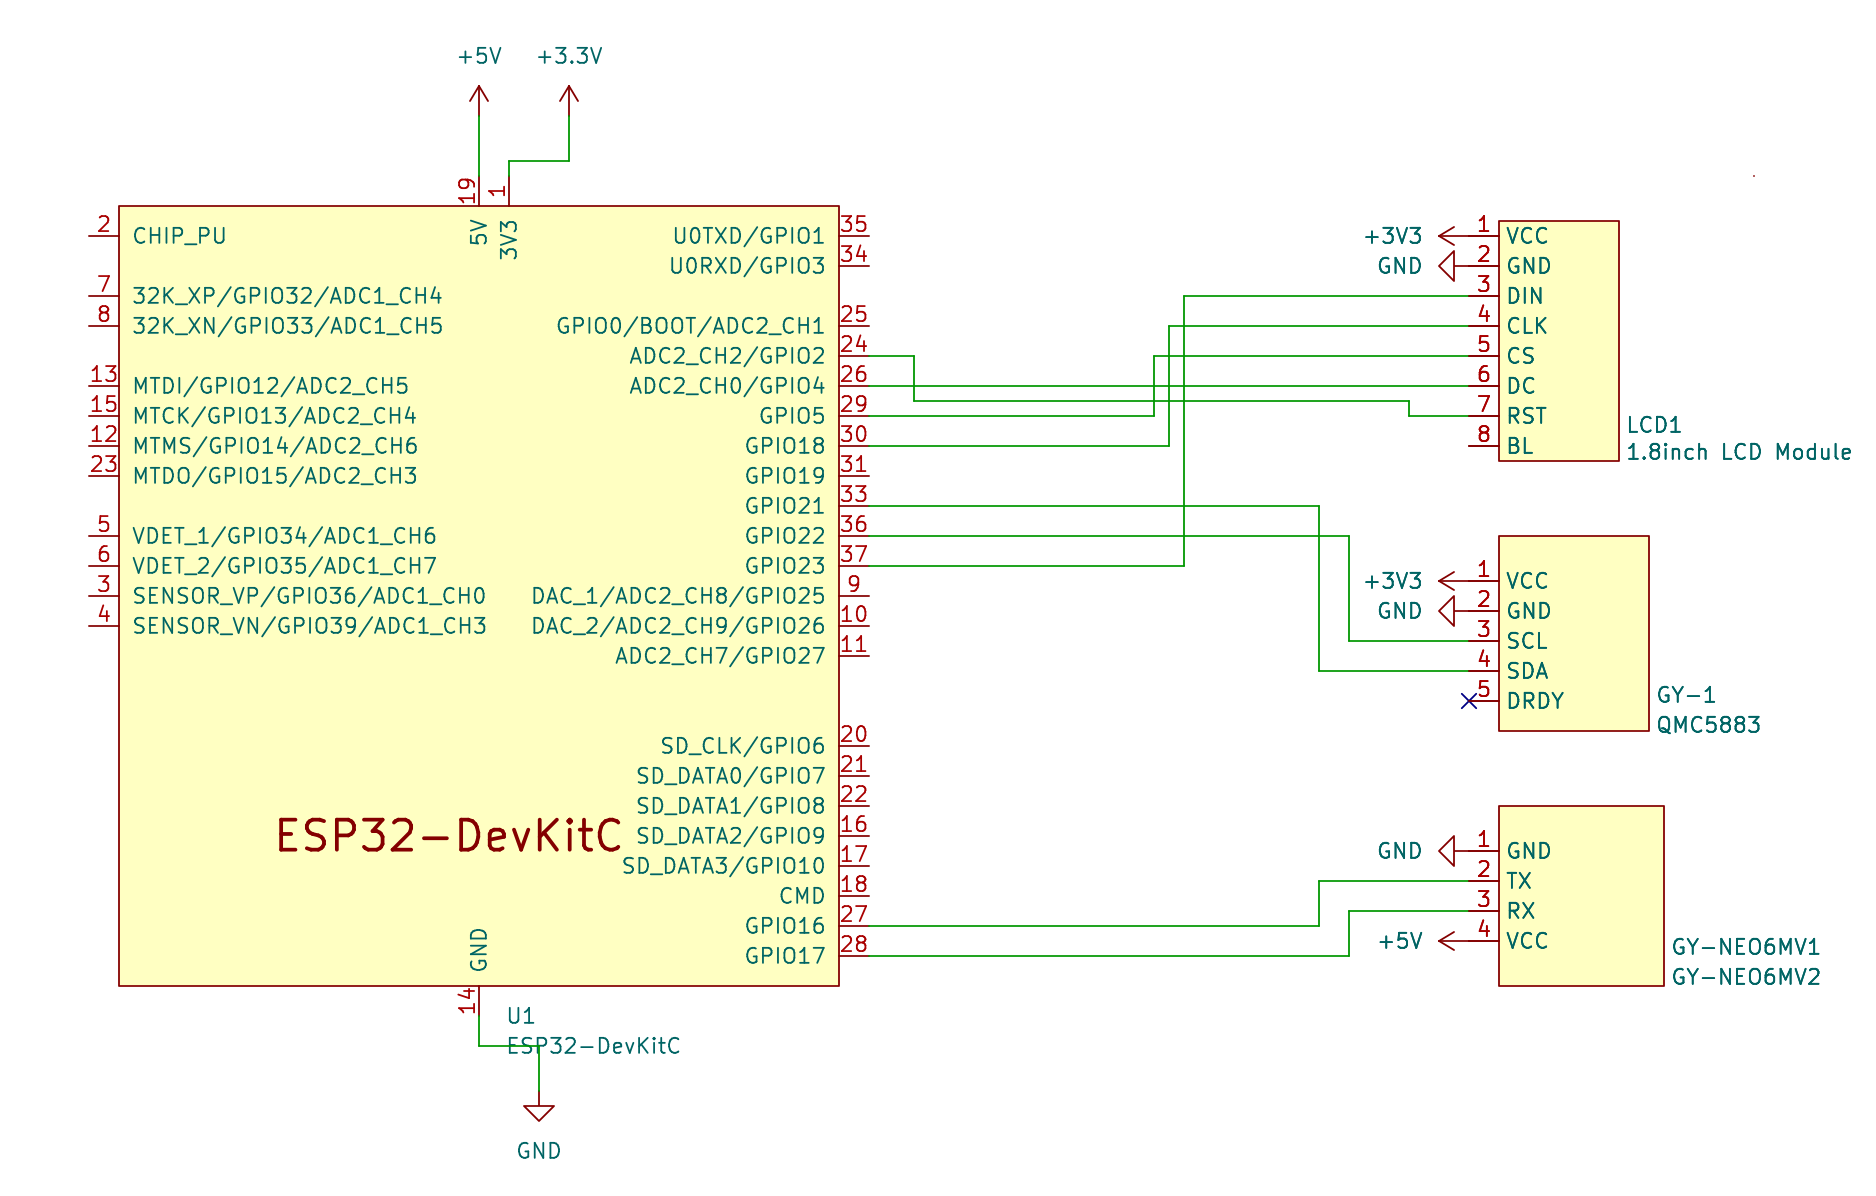
\includegraphics[width=0.75\linewidth]{hardware_schematics.png}
    \caption{Schemat prototypu urządzenia}
    \label{fig:scheme:hardware}
\end{figure}

\subsection{Kosztorys prototypu}
Kosztorys uwzględnia ceny głównych modułów urządzenia. Dotychczasowe koszty zostały pokryte przez członków grupy projektowej. Posiadamy również inne niezbędne części podstawowe, takie jak rezystory, kondensatory czy przyciski, które będą niezbędne przy testowaniu prototypu.

\begin{table}[h]
    \centering
    \begin{tabular}{|l|l|r|r|}
        \hline
        \textbf{Nazwa części} & \textbf{Typ}                 & \textbf{Cena detaliczna} & \textbf{Faktyczny koszt} \\ \hline
        Espressif DevKitV4    & ESP-WROOM-32E                & 35,99 zł                 & 35,99 zł                 \\ \hline
        GY-273                & Magnetometr cyfrowy 3-osiowy & 17,00 zł                 & 13,71 zł                 \\ \hline
        GY-NEO6MV2            & Moduł GPS z anteną           & 27,99 zł                 & 27,99 zł                 \\ \hline
        Waveshare 13892       & Wyświetlacz LCD 128x160px    & 33,90 zł                 & 0,00 zł                  \\ \hline
        \textbf{Razem}        &                              & \textbf{114,88 zł}       & \textbf{77,69 zł}        \\ \hline
    \end{tabular}
    \caption{Kosztorys prototypu}
\end{table}

\subsection{DevKitV4 ESP-WROOM-32E}

DevKitV4 ESP-WROOM-32E to zaawansowany moduł mikroprocesorowy z serii ESP32. Łączy w sobie  wysoką wydajność, niskie zużycie energii i wszechstronność. Wyposażony jest w podwójny rdzeń, obsługujący taktowanie do 240 MHz, oraz wbudowane Wi-Fi i Bluetooth. Posiada szeroki zakres interfejsów, zapewniając elastyczność w przypadku podłączania z modułami peryferyjnymi.

\subsection{LCD Waveshare 1.8inch 128x160}

Waveshare 1.8inch 128x160 to kolorowy wyświetlacz TFT o rozdzielczości 128x160 pikseli. Oferuje jasny i wyraźny obraz, umożliwiający wyświetlanie tekstu, grafiki i prostych animacji. Dane przesyłane są poprzez interfejs SPI.

\subsection{Mangetometr HMC5883L}

HMC5883L to trójosiowy magnetometr cyfrowy, który może mierzyć pole magnetyczne ziemi, co pozwala na określenie orientacji przestrzennej i wykorzystanie w roli kompasu. Dane odczytywane są poprzez interfejs I2C.

\subsection{GPS GY-NEO6MV2}

GY-NEO6MV2 to moduł GPS oparty na układzie NEO-6M, który umożliwia precyzyjne śledzenie pozycji geograficznej poprzez komunikację z satelitą za pomocą podłączonej anteny. Dane przezkazywane są poprzez standardowy interfejs UART.

\subsection{Napotkane problemy}

Podczas programowania oraz testowania komunikacji mikroprocesora z urządzeniami peryferyjnymi napotkano problemy z obsługą modułu GPS oraz magnetometru. \\

W przypadku połączenia z modułem GPS, wykryto wadliwość 2 z 4 zamówionych urządzeń - po wyznaczeniu oraz podłączeniu działających komponentów, nie wystąpiły już dalsze problemy. \\

W przypadku obsługi magnetometru pojawiały się problemy wydające się losowe w chwili próby nawiązania połączenia master-slave z modułem. Problemy te niekiedy zakłócały działanie całego programu załadowanego do mikroprocesora, niekiedy nie występowały, w innych przypadkach zaś powodowały błąd watchdoga w linii inicjalizacji sterownika I2C. Sterownik zawieszał się, oczekując transmisji na linii danych, które nigdy się nie pojawiały. Problem zidentyfikowano w błędzie implementacji sterownika I2C przez ESP-IDF. Użycie starszej wersji sterownika trwale usunęło problem. 

\section{Firmware}
Firmware aplikacji został napisany w języku C z wykorzystaniem platformy ESP-IDF \cite{esp-idf}.
ESP-IDF to oficjalne środowisko programistyczne dla platformy ESP32, które zawiera narzędzia do budowania, debugowania i wgrywania oprogramowania na urządzenie.

\subsection{Modularna struktura kodu} \label{sec:modularna-struktura-kodu}
Framework ESP-IDF pozwala na tworzenie projektów w sposób modułowy, co pozwala na łatwe dodawanie nowych funkcjonalności i niezależne testowanie poszczególnych komponentów.
W projekcie wyróżniono następujące moduły (komponenty):
\begin{itemize}
    \item \textbf{main} - moduł główny, inicjalizuje pozostałe moduły i definiuje zmienne współdzielone.
    \item \textbf{sc\_ble} - moduł odpowiedzialny za obsługę protokołu BLE. Zawiera definicje usług i charakterystyk GATT.
    \item \textbf{sc\_gps} - moduł obsługujący moduł GPS. Zawiera funkcje do odczytu współrzędnych geograficznych.
    \item \textbf{sc\_compass} - moduł obsługujący magnetometr. Zawiera funkcje do odczytu kierunku kompasu.
    \item \textbf{sc\_display} - moduł obsługujący wyświetlacz LCD. Zawiera funkcje do wyświetlania informacji na ekranie z wykorzystaniem biblioteki LVGL.
    \item \textbf{sc\_logic} - moduł odpowiedzialny za logikę aplikacji. Zawiera funkcje do obliczania kierunku i dystansu do celu.
    \item \textbf{lvgl} - moduł zawierający bibliotekę LVGL. \cite{lvgl-esp32-port} Zawiera konfigurację i funkcje pomocnicze do obsługi wyświetlacza.
    \item \textbf{lvgl\_esp32\_drivers} - moduł zawierający sterowniki dla ESP32 do biblioteki LVGL. \cite{lvgl-esp32-drivers}
\end{itemize}

\subsection{Architektura wielowątkowa}
Framework ESP-IDF jest oparty na architekturze FreeRTOS \cite{freertos-docs}, co pozwala na tworzenie wielowątkowych aplikacji.
Zawarta we frameworku wersja FreeRTOS pozwala na wykorzystanie dwóch rdzeni procesora ESP32, zapewniając równoległe wykonywanie zadań w dwóch wątkach.
Każdy z modułów aplikacji opisanych w sekcji \ref{sec:modularna-struktura-kodu} działa w osobnym wątku.

\subsubsection{Zmienne współdzielone}
Program zawiera dwie zmienne współdzielone odpowiedzialne za przechowywanie aktualnych danych na temat odczytów z sensorów oraz przechowywanie aktualnych danych do wyświetlenia na ekranie.

\begin{lstlisting}[language=C, caption=Definicja zmiennej dla odczytów sensorów]
typedef struct {
    SemaphoreHandle_t mutex;
    compass_position_t position;
    float bearing; // in radians
    float bearing_deg; // in degrees
    compass_path_t path;
    bool position_updated;
} compass_data_t;
\end{lstlisting}

\begin{lstlisting}[language=C, caption=Definicja zmiennej dla danych wynikowych]
typedef struct {
    SemaphoreHandle_t mutex;
    // Angle in 0.1 degrees - between 0 and 3600
    int16_t angle;
    // Next waypoint id
    uint16_t next_wp;
    // Distance to next waypoint in meters
    uint32_t distance;
    bool finished;
} display_data_t;
\end{lstlisting}

Każda zmienna posiada semafor, który zapewnia dostęp do zasobu w sposób atomowy, co zapobiega konfliktom między wątkami.



\subsection{Protokół komunikacji Bluetooth Low Energy (BLE)}
Protokół komunikacji BLE został zaimplementowany zgodnie ze standardem Bluetooth Core 4.2 \cite{bluetooth-core-spec-4-2} na platformie ESP32.
Użyto stosu i ESP-NimBLE \cite{esp-idf-nimble-docs}, który zapewni odpowiednie zarządzanie pamięcią oraz obsługę komunikacji BLE.
Stos ESP-NimBLE jest alternatywną wersją stosu Apache MyNewt Nimble \cite{apache-mynewt-docs}, przystosowaną do pracy z mikrokontrolerami producenta Espressif.

\subsubsection{Obsługa po stronie urządzenia}
Urządzenie wykorzystuje stos ESP-NimBLE do implementacji protokołu BLE, co pozwala na zmniejszenie zużycia pamięci.
Komunikacja z aplikacją mobilną opiera się na deklaracji usług i charakterystyk GATT, umożliwiając przesyłanie danych trasy w postaci tablic par współrzędnych geograficznych.

\begin{lstlisting}[language=C, caption=Definicja charakterystyki GATT]
static uint8_t gatt_svr_chr_val[MAX_CHAR_LEN];
static uint16_t gatt_svr_chr_val_handle;
static const ble_uuid128_t gatt_svr_chr_uuid =
        BLE_UUID128_INIT(0x00, 0x00, 0x00, 0x00, 0x11, 0x11, 0x11, 0x11,
                         0x22, 0x22, 0x22, 0x22, 0x33, 0x33, 0x33, 0x33);
\end{lstlisting}


\subsection{Napotkane problemy}
W trakcie rozwoju oprogramowania pojawiły się dwa główne problemy opisane w poniższych podrozdziałach.
\subsubsection{Konflikty między bibliotekami}
W trakcie rozwoju modułu odpowiedzialnego za komunikację z wyświetlaczem LCD pojawił się konflikt między:
\begin{itemize}
    \item Frameworkiem ESP-IDF
    \item Biblioteką LVGL,\cite{lvgl-esp32-port} która jest prostym silnikiem GUI
    \item Biblioteką LVGL ESP32 Drivers, \cite{lvgl-esp32-drivers} która zawiera sterowniki dla ESP32 do biblioteki LVGL
\end{itemize}
Początkowe próby integracji wszystkich trzech bibliotek w najnowszej wersji nie powiodły się,
co skutkowało koniecznością doboru kompatybilnych wersji bibliotek oraz dostosowaniem konfiguracji.
Proces naprawy konfliktów trwał kilka dni.

\subsubsection{Błąd w implementacji protokołu I2C w bibliotece ESP-IDF}
Do komunikacji z magnetometrem QMC5883 wykorzystano interfejs I2C \textit{(Inter Integrated Circut)}, który jest standardowym interfejsem komunikacyjnym dla urządzeń peryferyjnych.
Producent mikrokontrolera ESP32, firma Espressif, dostarcza bibliotekę do obsługi interfejsu I2C w ramach frameworku ESP-IDF.

W trakcie implementacji okazało się, że biblioteka ESP-IDF zawiera błąd w implementacji protokołu I2C, który uniemożliwiał poprawną komunikację z magnetometrem.
Dodatkowo, bład ten był niewykrywalny w procesie debugowania, co nie pozwalało na jednoznaczne zlokalizowanie problemu (mógł wynikać z błędu w kodzie, konfiguracji, podłęczeniu lub z uszkodzenia magnetometru).

Błąd naprawiono poprzez zastosowanie alternatywnej biblioteki do obsługi interfejsu I2C, co pozwoliło na poprawną komunikację z magnetometrem.

\section{Aplikacja mobilna}
Aplikacja mobilna spełnia następujące funkcjonalności:
\begin{itemize}
    \item rysowanie tras
    \item zapisywanie tras
    \item zarządzanie trasami
    \item nawiązywanie połączenia z urządzeniem SmartCompass
    \item przesyłanie tras do urządzenia SmartCompass
\end{itemize}

\subsection{Wykorzystane technologie}
Aplikacja została zrealizowana przy użyciu frameworku \textbf{React Native} \cite{react-native-docs} pozwalającego tworzyć jeden projekt, który następnie kompilowany jest do kodu aplikacji wykonywalnej na urządzeniach z Androidem jak i iOS. Ze względu na wymagania powiązane z uzyskaniem dostępu do modułu Bluetooth Low Energy urządzenia, zadecydowaliśmy się rozwijać naszą aplikację jedynie w kierunku systemu Android.
Ponadto wykorzystano platformę i zestaw narzędzi \textbf{Expo} \cite{expo-docs}, które upraszczają proces tworzenia, testowania i wdrażania aplikacji mobilnych.

\subsection{Wykorzystane biblioteki}

W aplikacji wykorzystano szereg bibliotek, które ułatwiły realizację poszczególnych funkcjonalności:

\begin{itemize}
    \item \textbf{react-native-async-storage} - Służy do przechowywania danych lokalnych na urządzeniu. Umożliwia łatwe zapisywanie i odczytywanie danych, takich jak ustawienia użytkownika czy trasy.
    \item \textbf{react-navigation} - Biblioteka do nawigacji w aplikacjach React Native. Umożliwia łatwe zarządzanie stosami ekranów, nawigację pomiędzy nimi oraz implementację różnorodnych wzorców nawigacji.
    \item \textbf{react-native-ble-plx} - Biblioteka do obsługi Bluetooth Low Energy (BLE). Umożliwia skanowanie, łączenie i komunikację z urządzeniami BLE, co jest kluczowe dla integracji z urządzeniem SmartCompass.
    \item \textbf{react-native-quick-base64} - Umożliwia szybkie kodowanie i dekodowanie danych w formacie base64, co jest przydatne przy przesyłaniu danych przez BLE.
    \item \textbf{react-native-vector-icons} - Biblioteka dostarczająca zestaw ikon do aplikacji. Umożliwia łatwe dodawanie ikon do przycisków, menu i innych elementów interfejsu użytkownika.
    \item \textbf{react-native-maps} - Biblioteka do integracji map w aplikacji. Umożliwia wyświetlanie map, rysowanie tras oraz interakcję z punktami na mapie.
    \item \textbf{react-native-reanimated} - Biblioteka do tworzenia płynnych i wydajnych animacji w aplikacji. Umożliwia tworzenie zaawansowanych animacji i interakcji, co poprawia ogólne wrażenia użytkownika.
\end{itemize}

\subsection{Tworzenie wersji \textit{release} aplikacji}
Pierwszym krokiem jest dodanie informacji takich jak nazwa, ikona, splash screen oraz konfiguracje specyficzne dla platformy Android do pliku \texttt{app.json}.

\begin{lstlisting}[caption=Plik app.json]
"expo": {
    "name": "app",
    "slug": "app",
    "version": "1.0.0",
    "orientation": "portrait",
    "icon": "./assets/icon.png",
    "plugins": [
      "react-native-ble-plx"
    ],
    "userInterfaceStyle": "light",
    "splash": {
      "image": "./assets/splash.png",
      "resizeMode": "contain",
      "backgroundColor": "#ffffff"
    },
}
\end{lstlisting}

należy również utworzyć konfigurację dla usługi \textbf{Expo Application Services (EAS)}, który jest częścią procesu budowania aplikacji. Konfigurację tą umieszcza się w pliku \texttt{eas.json}.

\begin{lstlisting}[caption=Plik eas.json]
{
  "cli": {
    "version": ">= 8.0.0"
  },
  "build": {
    "development": {
      "developmentClient": true,
      "distribution": "internal"
    },
    "preview": {
      "android": {
        "buildType": "apk"
      }
    },
    "production": {}
  },
  "submit": {
    "production": {}
  }
};
\end{lstlisting}

Dla klucza \texttt{preview} określamy typ budowania aplikacji jako \texttt{"apk"} dla platformy Android.
Następnie należy zalogować się do konta \textit{Expo}, a później, korzystając z komendy \texttt{'npx build -p android –profile preview'}, wygenerować plik \texttt{.apk}, który dostępny będzie do pobrania z konta użytkownika w platformie \textit{Expo}. Proces generowania pliku \texttt{.apk} jest zautomatyzowany i przeprowadzany przez narzędzie \textbf{Expo Build Service}. W przypadku naszej aplikacji rozwiązanie to znacząco ułatwia cały proces względem \textit{Bare Workflow}, czyli podejścia w którym nie wykorzystuje się frameworka \textit{Expo}.

\subsubsection{Różnice pomiędzy wersją testową, a \textit{release}}
Wersje testowe i release różnią się znacząco pod względem celu, konfiguracji, procesu budowania oraz dystrybucji. Wersje testowe są przeznaczone do szybkich iteracji i debugowania, zawierając narzędzia deweloperskie i umożliwiając natychmiastowe aktualizacje. Wersje release są zoptymalizowane pod kątem wydajności, stabilności i bezpieczeństwa, przeznaczone do dystrybucji do szerokiego grona użytkowników końcowych poprzez oficjalne sklepy aplikacji.

\subsection{Napotkane problemy}
Obsługa połączenia BLE z urządzeniem okazała się być trudniejsza niż zakładaliśmy, w szczególności monitorowanie sesji z poziomu aplikacji mobilnej. Cały proces wymaga również uzyskania odpowiednich pozwoleń od urządzenia na którym działa aplikacja, a proces testowania był utrudniony ponieważ posiadamy tylko jeden egzemplarz urządzenia SmartCompass. Ze względów technicznych UUID serwisu BLE naszego urządzenia SmartCompass został na sztywno ustawiony w aplikacji.